\begin{IEEEbiography}
[{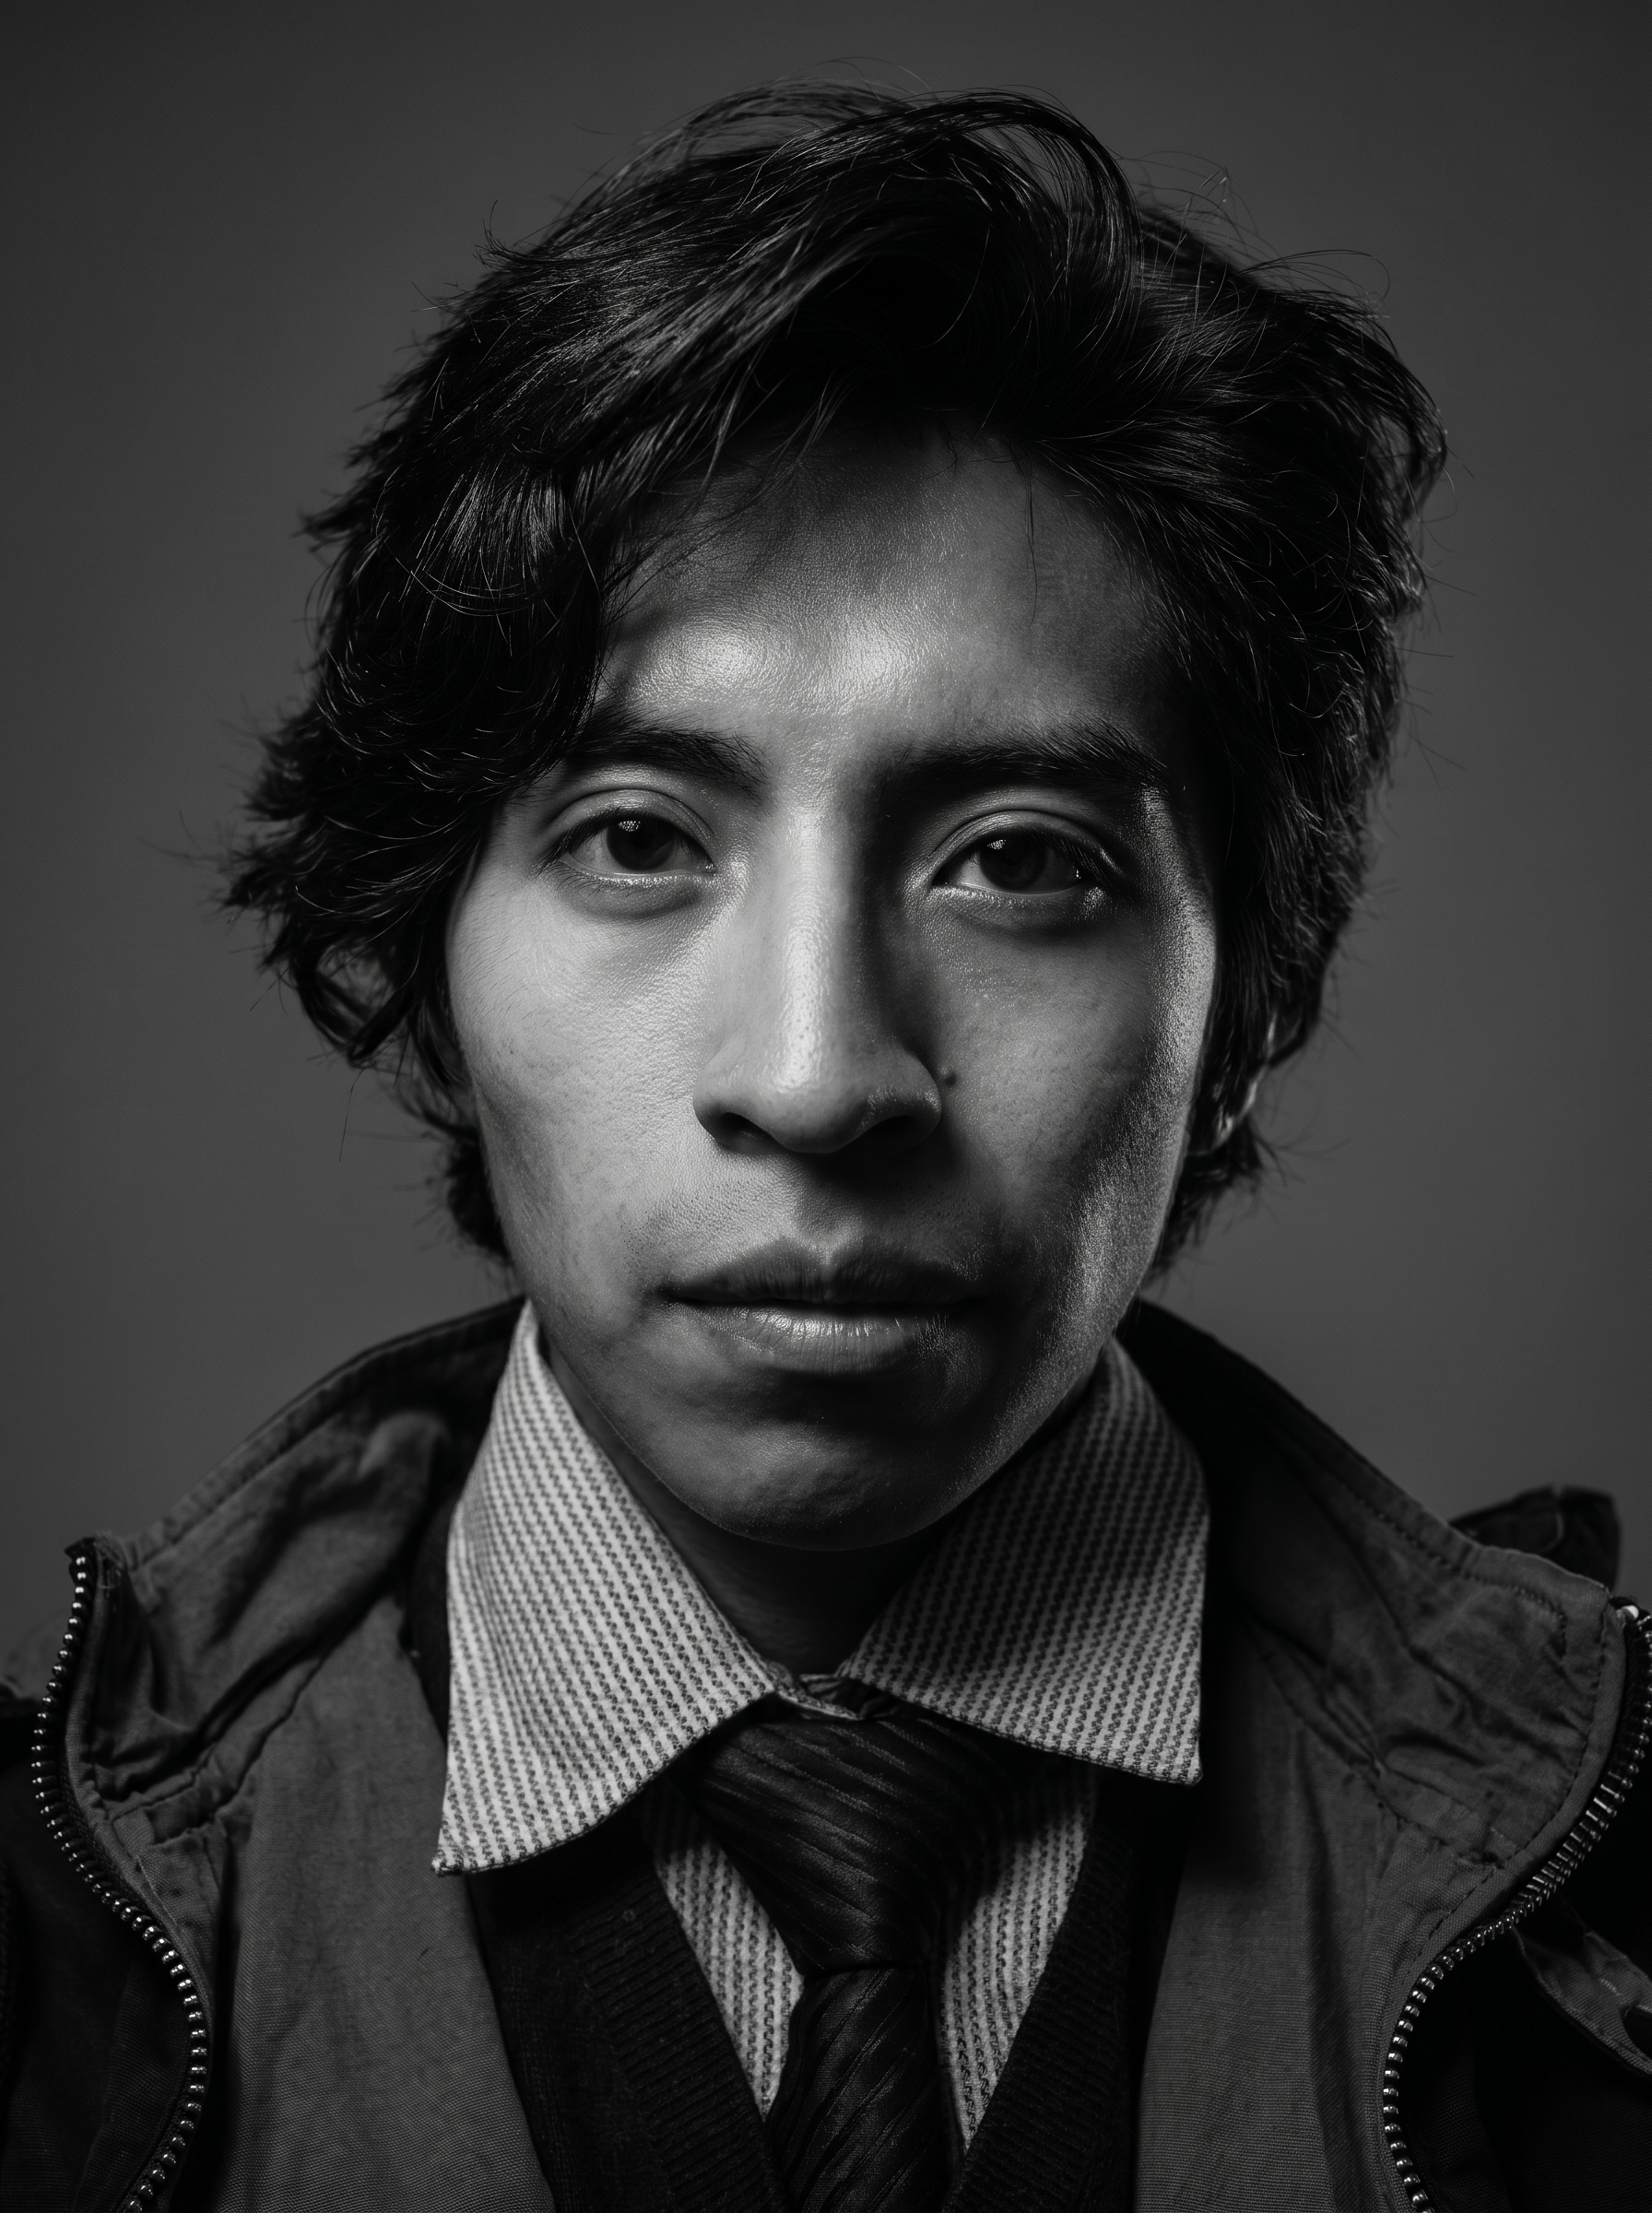
\includegraphics[width=1in,height=1.25in,clip,keepaspectratio]{images/Byron.jpeg}}]{Byron Paul Condolo Narvaez}
es estudiante de pregrado de la carrera de Computación en la Facultad de Ingeniería y Ciencias Aplicadas de la Universidad Central del Ecuador (UCE). Realiza este proyecto de simulación de WannaCry en redes locales como parte de su formación académica en la cátedra de simulación y sistemas colaborativos.
\end{IEEEbiography}

\begin{IEEEbiography}
[{
\includegraphics[width=1in,height=1.25in,clip,keepaspectratio]{images/Kelly.jpeg}}]{Kelly Denisse Ledesma Aguilar}
es estudiante de pregrado de la carrera de Computación en la Facultad de Ingeniería y Ciencias Aplicadas de la Universidad Central del Ecuador (UCE). Participa en este estudio de propagación y modelado multiagente BDI como parte de su desarrollo académico práctico y aprendizaje en ciberseguridad y redes informáticas.
\end{IEEEbiography}

\begin{IEEEbiography}
[{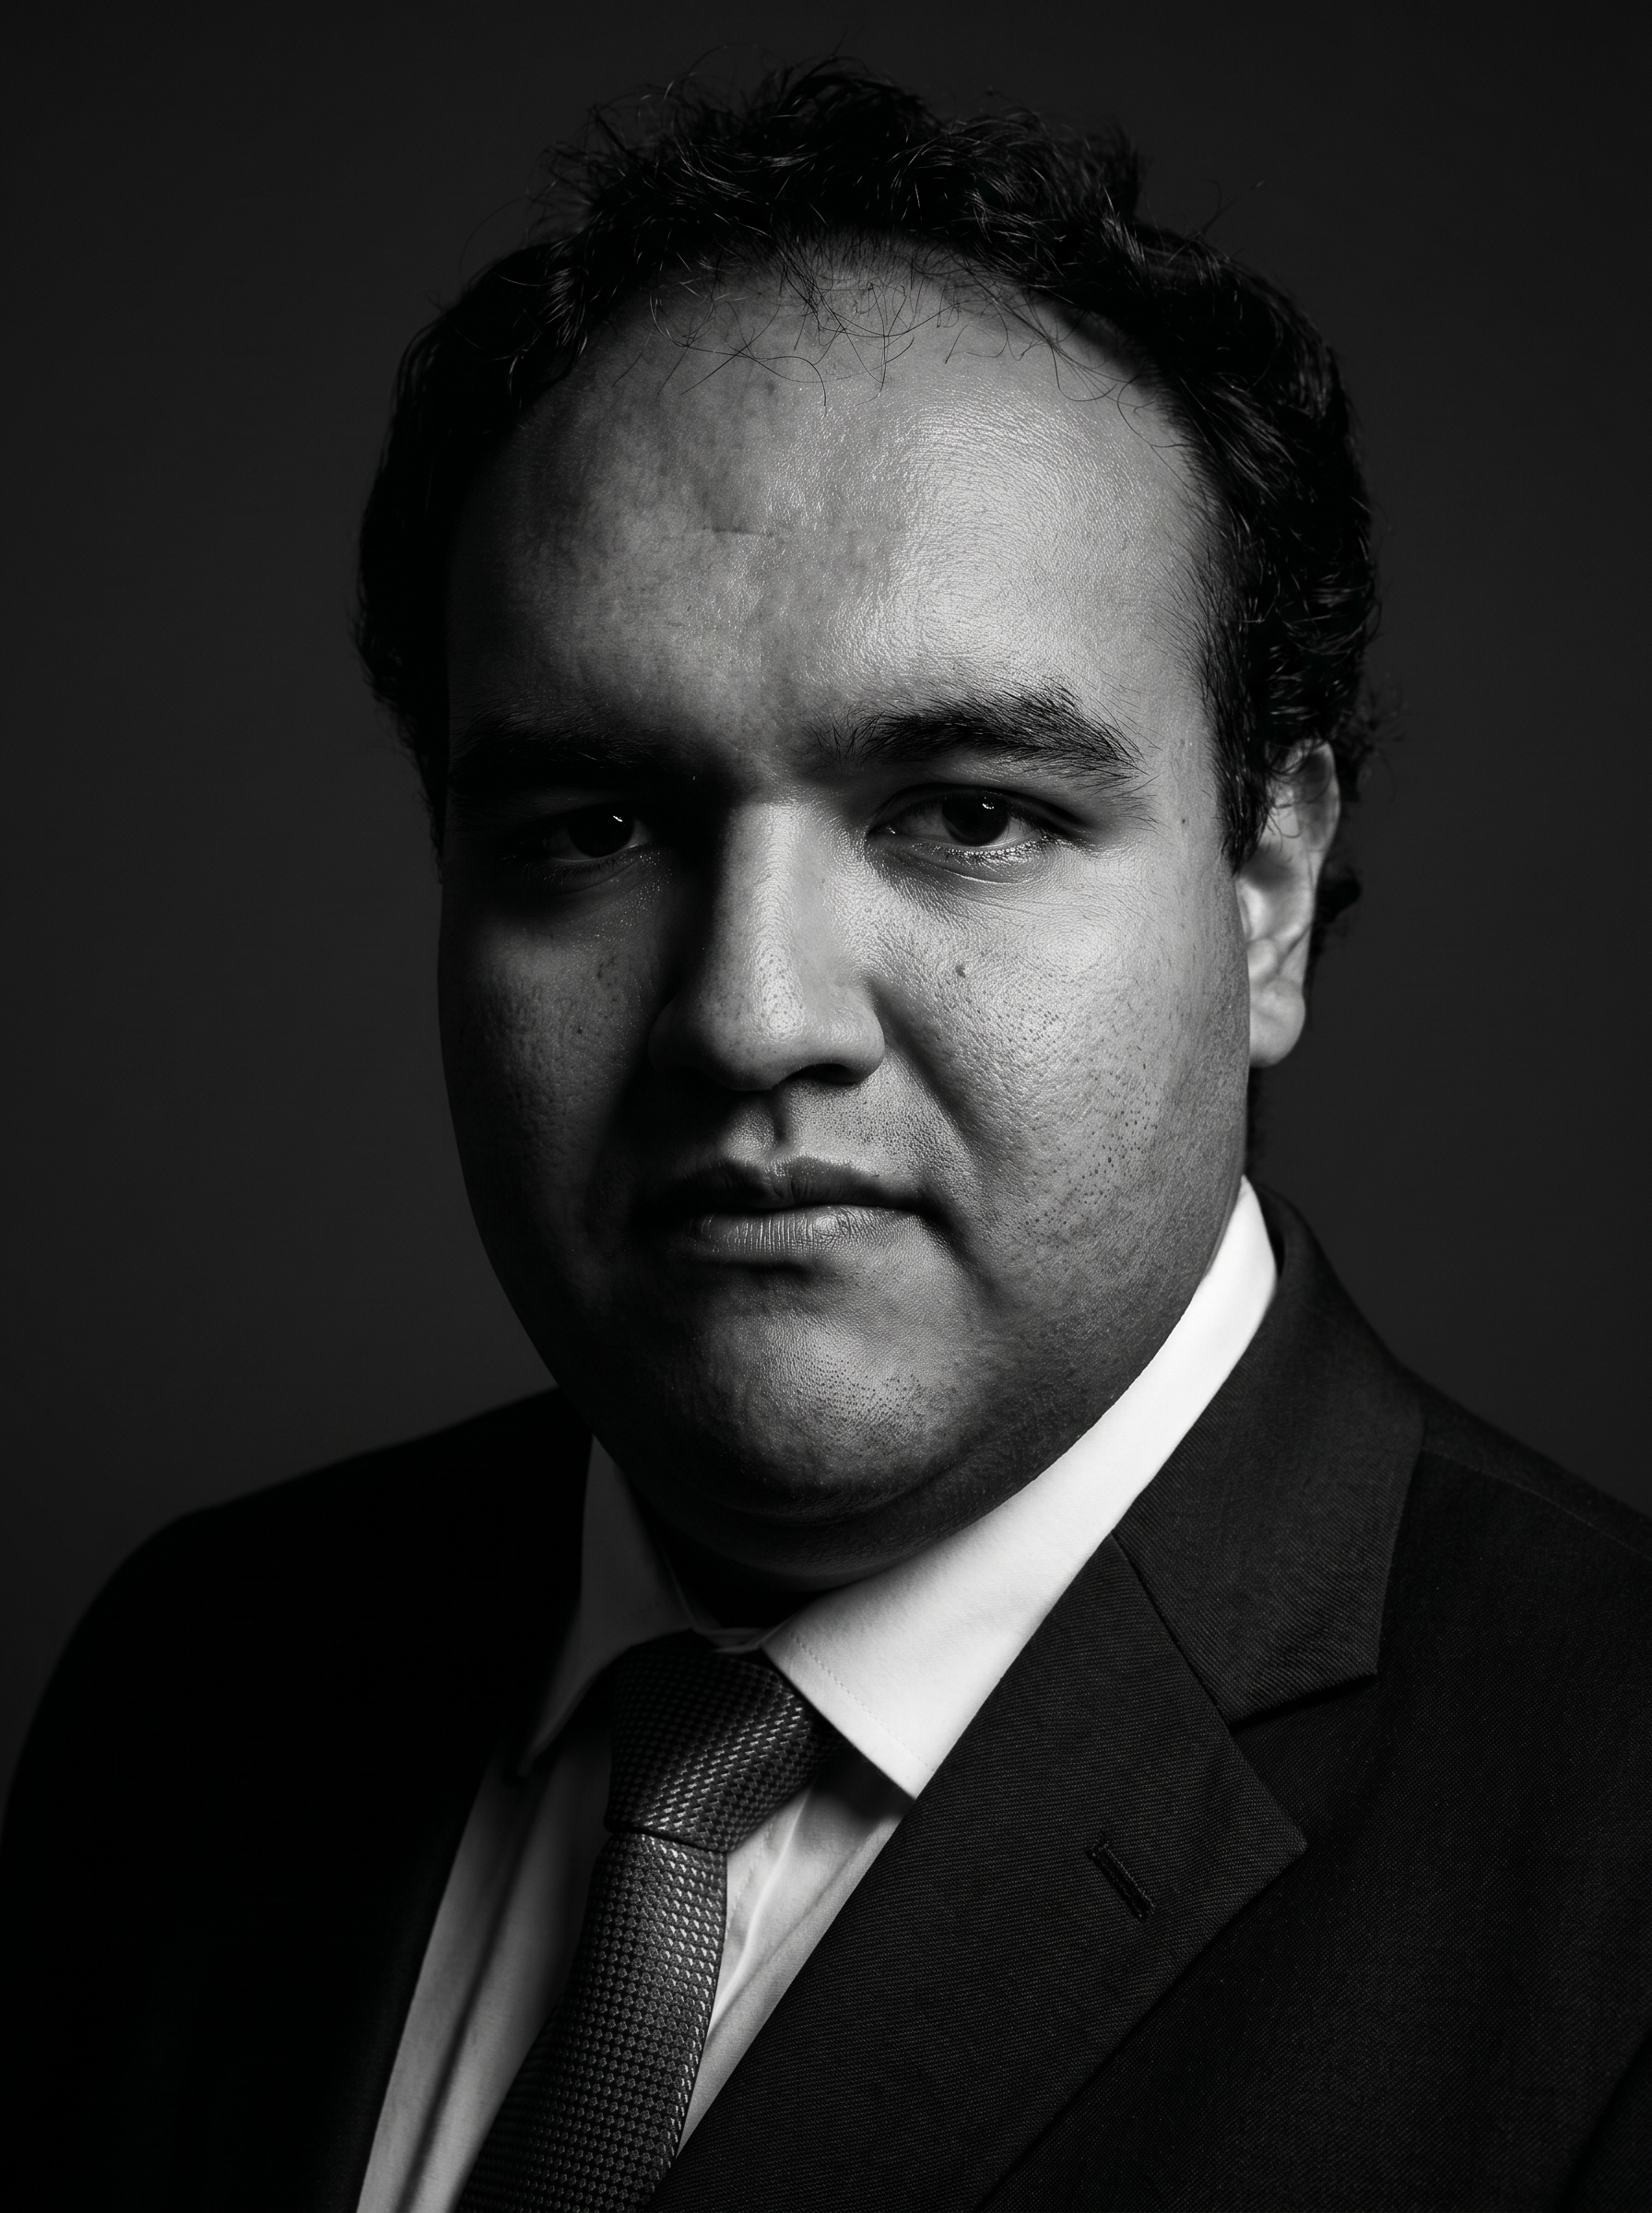
\includegraphics[width=1in,height=1.25in,clip,keepaspectratio]{images/Bryan.jpeg}}]{Bryan Eduardo Loya Cadena}
es estudiante de pregrado de la carrera de Computación en la Facultad de Ingeniería y Ciencias Aplicadas de la Universidad Central del Ecuador (UCE). Desarrolla este modelo colaborativo y dashboard en Vue 3 con el fin de fortalecer sus conocimientos académicos prácticos en desarrollo frontend y simulación de sistemas distributivos complejos.
\end{IEEEbiography}

\begin{IEEEbiography}
[{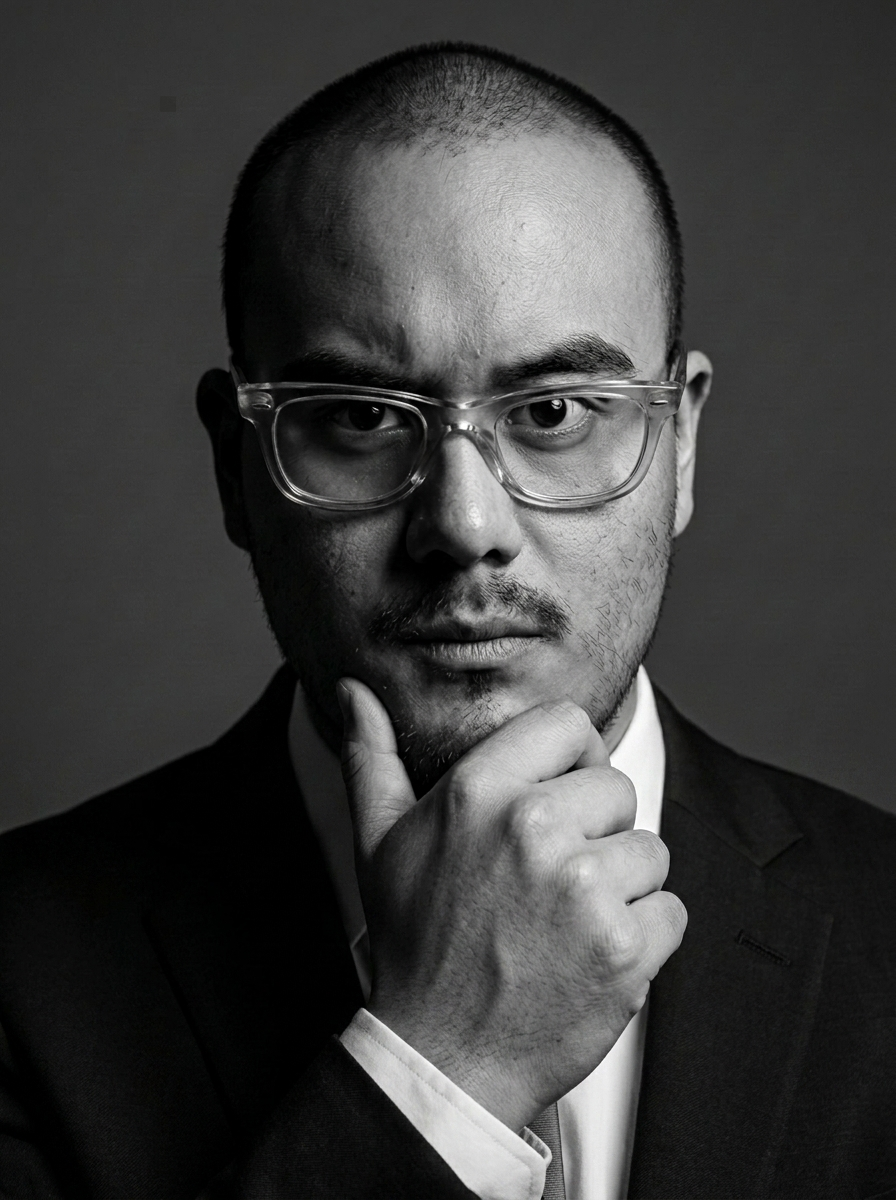
\includegraphics[width=1in,height=1.25in,clip,keepaspectratio]{images/Dennis.jpeg}}]{Dennis Adrian Trujillo Vistin}
es estudiante de pregrado de la carrera de Computación en la Facultad de Ingeniería y Ciencias Aplicadas de la Universidad Central del Ecuador (UCE). Contribuye al diseño del modelo BDI y a la integración de datos geográficos de red como parte de sus trabajos de simulación de redes locales y ciberseguridad a nivel universitario.
\end{IEEEbiography}
